\chapter{SynVisio}

Our biggest contribution in this research was the development of SynVisio an online platform to explore syteny by mapping syntenic blocks that are highly conserved and long enough to be significant between a given pair of genomes or within a single genome.In this chapter we first describe the different modes SynVisio offers for syteny analysis and how each one operates.We then explore the different features SynVisio provides to enhance user experience with the tool.Following this we discuss the implementation of the tool and the choices made regarding its web architecture and visual design.Finally we look at a  usage scenario through a series of steps depicting how SynVisio can be used to explore the genomic conservation between a sample data-set of humans and chimpanzees.

\section{System Overview}
SynVisio is a multi scale genome browser that can be accessed through the web and lets researchers explore genomic conservation.It lets researchers upload the synteny files of their choice and generates visualizations on demand from the information in these files.It offers two analysis modes : Single Level and Multi Level.In the first mode users can compare genomes two at a time through a dashboard where syteny is visualized as both a dot plot and a linear connector plot.The charts are accompanied by a filter panel where the conserved genomic blocks can be filtered based on various features such as degree of similarity.In the second mode researchers can compare several genomes at a time through hive plots or stacked linear plots.To aid researchers in their visual exploration of synteny,SynVisio lets them annotate the generated charts with additional tracks in the form of histograms, heat-maps or other basic plots.Additional features are also provided such as a gene search panel to look for specific genes and the ability to export generated charts for publication.

\section{Analysis Mode}
Gene sequences can be compared in different ways depending on the underlying biological question.Which means syteny analysis can vary between visualizing simple pairwise matches between two genomes to preforming multi way comparisons across several genomes at once.The availability of datasets and their inherent quality also plays into the kind of analysis that can be done.Whole genome alignment for example is usually done pairwise as looking for matches can be faster when the subset of available matches is low.Additionally in the context of Synteny detection which is anchor   based, identifying common markers between multiple genomes is difficult.However when the data is available, multi way comparisons can offer better insights and tackle bigger questions like pan genome syteny.Thus SynVisio offers both a Single and a Multi Level analysis mode depending on the the researchers choice and the data availability.

\subsection{Single Level Analysis}
This is default mode in which SynVisio operates and is meant for exploratory tasks as it presents the collinearity between a selected set of chromosomes in two different visual representations and lets users filter the collinear blocks on the fly.

\begin{figure}
  \centering
  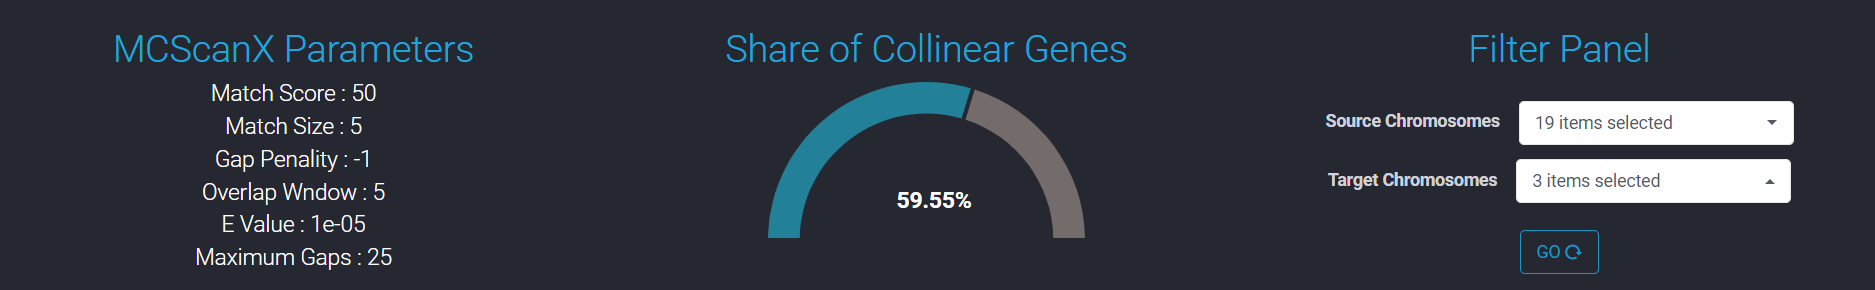
\includegraphics[width=1\linewidth]{images/ch_4_baseparameters.PNG}
  \captionof{figure}{Synteny detection parameters and level of collinearity presented along with toggles to select source and target chromosomes.}
  \label{fig:ch_4_baseparameters}
\end{figure}


The first step involved in using the dashboard is providing an input dataset, for this, users can either upload their own datasets or use existing sample files.We have already processed several datasets depicting genome conservation that are available on the homepage of our application and are adding more every month.Some of the examples include self syteny in Brassica napus(canola), cross syteny between Oriza satica(rice) and Sorghum bicolor(broom-corn) and cross syteny between Arabidopsis thaliana(thale cress) and Vitis vinifera(grape vine).After the intial data uploading and processing stage is complete basic information about the parameters used in the syteny detection process are presented along with the percentage share of collinearity present in the files accompanied with toggles to select the source and target chromosomes as shown in Figure \ref{fig:ch_4_baseparameters}.The list of chromosomes are ordered alpha-numerically to divide the different species into distinct groups and make it easier to pick chromosomes sequentially.

To visualize genomic conservation we adopted a design based on the popular Visual Information Seeking Mantra \cite{Shneiderman96theeyes} which is made of the seven tasks: overview, zoom, filter, details-on-demand, relate, history and extract.Our design presents the information in a top down approach in three distinct levels.At the first level users are given the option to  compare genomes by selecting all or a specific subset of chromosomes between the source and the target genome which in cases of self syteny is the same genome.This level is called the whole genome level and consists of two visualizations(a,b) accompanied by a inner filter panel(c) as shown in Figure \ref{fig:ch_4_dashboard}. 


% refer to paper on linked views and add more lierature 
% State of the Art:
% Coordinated & Multiple Views in Exploratory Visualization
% Jonathan C. Roberts
% Computing Laboratory, University of Kent, UK
% j.c.roberts@kent.ac.uk


The first visualization on the top is a linear link plot where syntenic collinear blocks are connected by coloured ribbons as shown in Figure.The source chromosomes are laid out on the top and the target chromosomes are spread out in the bottom.The size of the chromosomes are calculated based on the genomic sizes of the chromosomes and the available screen width to ensure that the visualizations are responsive across different screen-sizes.Chromosomes in the source layer are coloured using a chromatic 10 point color scale derived from ColorBrewer\cite{colorbrewer} and are set to repeat after every 10th chromosome.The choice to limit the colours to 10 was made humans and the chromosomes in the target layer are coloured in an alternating grey scale.Collinear blocks are then coloured based on their source target chromosome colour so that they can be visually distinct from the other blocks.

\begin{figure}
  \centering
  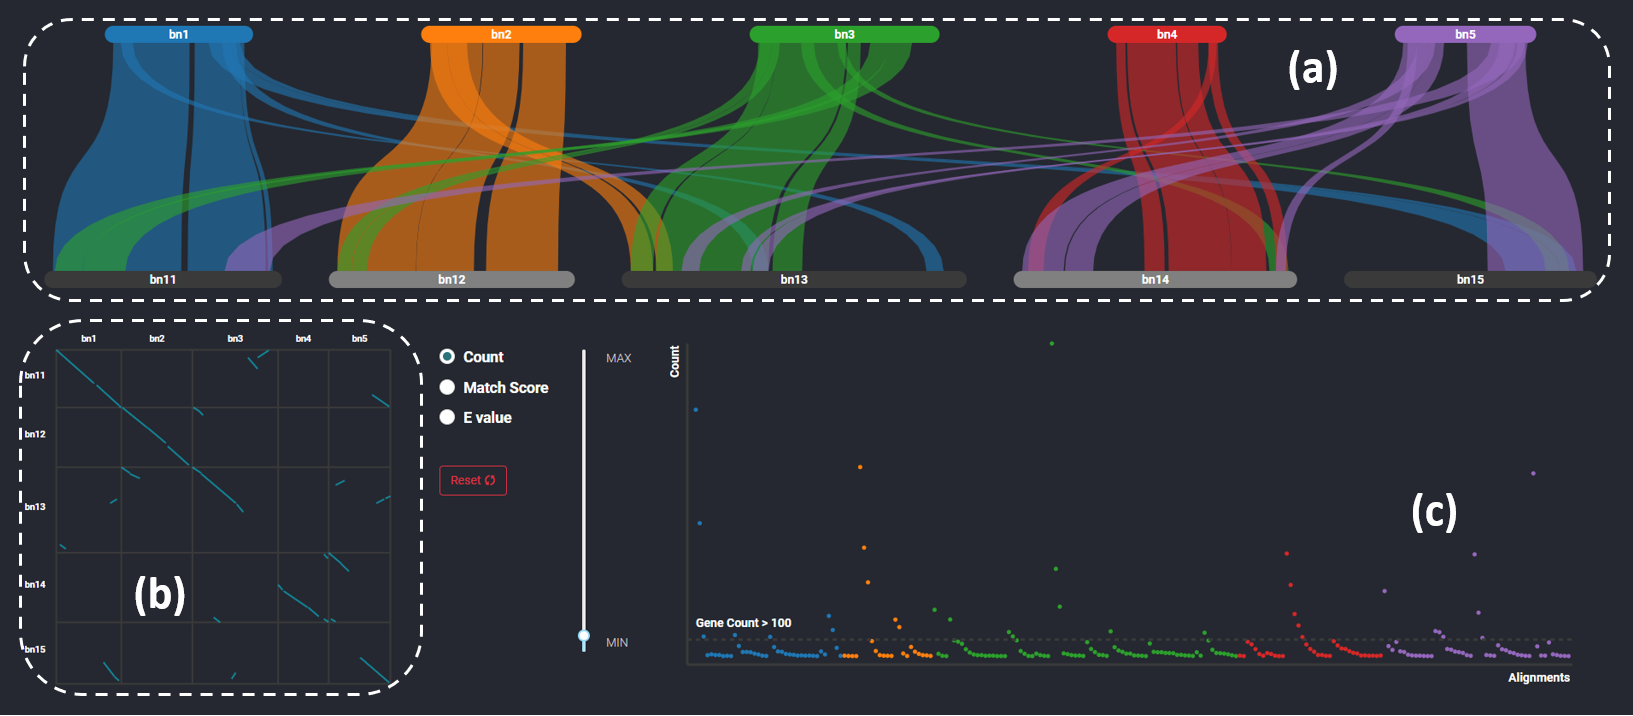
\includegraphics[width=.75\linewidth]{images/ch_1_dashboard.PNG}
  \captionof{figure}{Single analysis mode visualizing genome collinearity in Bn(Brassica Napus) with the following components: \textbf{a)} Linear Link Plot with connected ribbons representing collinear gene blocks. \textbf{b)}Dot plot where every collinear gene is represented by a point and contiguous collinear blocks are shown as lines. \textbf{c)} Filter panel representing all the collinear blocks based on the count of their genes with ability to refine results using slider to the left.  }
  \label{fig:ch_4_dashboard}
\end{figure}


% For uploading their own datasets users need to provide two files, a collinearity file that is generated using a syteny detection software like MCScanX or DAGChainer containing the list of collinear blocks and a GFF file for the positions of all the reference genes in the genome.


% In this Mode SynVisio operates as a dashboard by default and presents genome collinearity in multiple representations.Users however have the choice to switch the visual representation using the configuration page and options available are a dot plot,a linear connector plot, and an exploratory dashboard with both plots and a filter panel.


% First talk about parameters and overall percentage share between source and target. and why its shown
% then filter panel why we select chromesome differe source and target. why they are sorted apla nuerically

% then we talk about the linear link plot then dot plot.
% then the filter panel why we need it..why the different features. why the slider. choice of colours at this stage.

% then chromosome mode .different colour for inversions then the ability to zoom and hover over links to see what they contain.

% then individual block mode then invert entire chromosome. then shift axis to right or zoom.



\subsection{Multi Level Analysis}
Hive Plots and Stacked Bar plots

\section{Usability Features}
\subsection{Track Annotation}
\subsection{Re-visitation Support}
\subsection{Gene Search Panel}
\subsection{Image Export}


\section{Usage Scenario}
A series of pictures explaining a particular exploratory scenario - Best done with Wheat genome showing genome triplication and further interlocation of some chromosomes.